% ============================================================================
% Section 9: Comparison with Existing Theories
% ============================================================================

\section{Comparison with existing theories}
\label{sec:comparison}

UHM is not the only mathematical theory of consciousness. To situate it
precisely, this section provides a systematic comparison with the six
leading frameworks: Integrated Information
Theory (IIT 4.0)~\cite{iit4}, Global Neuronal Workspace Theory
(GNWT)~\cite{dehaene2011}, the Free Energy Principle (FEP)~\cite{friston2019},
Higher-Order Theories (HOT)~\cite{lau2011}, Hoffman and Prakash's Conscious Realism
and Conscious Agent Theory (CAT)~\cite{hoffman2014}, and Worden's recently proposed
Projective Wave Theory (PWT)~\cite{worden2026}.

\begin{figure}[H]
\centering
% Comparison Radar/Table: UHM vs IIT vs GWT vs FEP vs HOT
% Visual comparison of theory capabilities

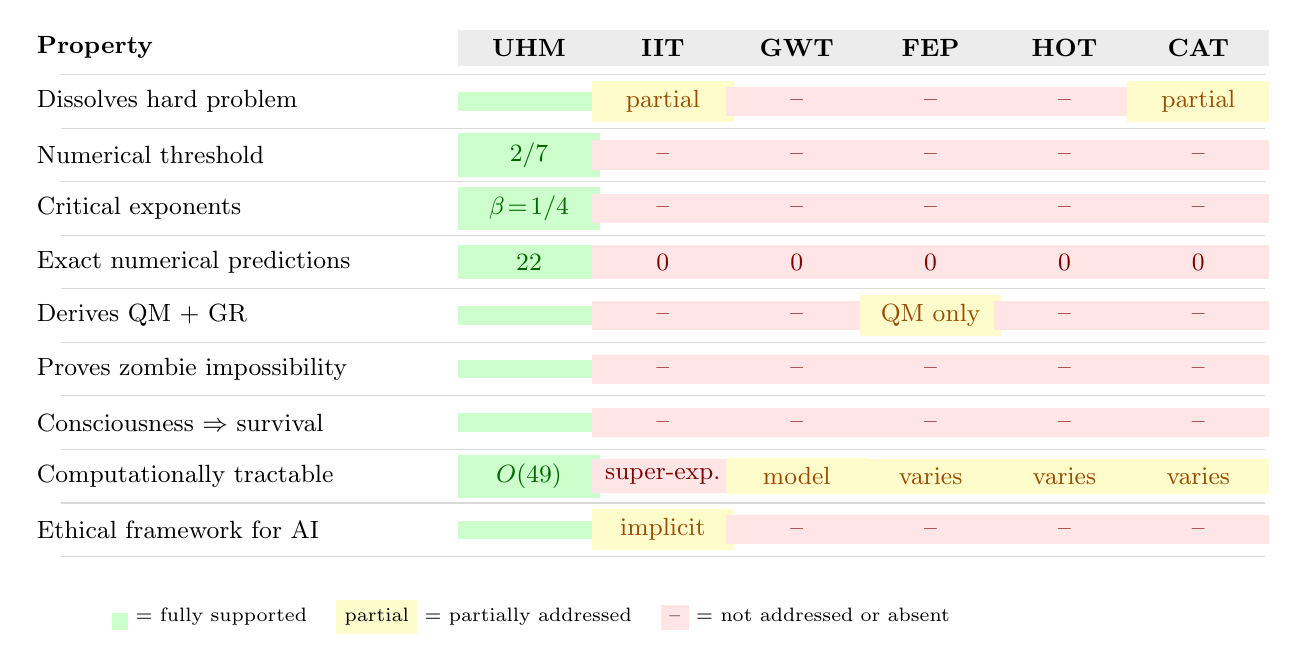
\begin{tikzpicture}[
  score/.style={font=\small, minimum width=1.8cm, align=center},
  yes/.style={score, fill=green!20, text=green!40!black},
  partial/.style={score, fill=yellow!20, text=orange!60!black},
  no/.style={score, fill=red!10, text=red!50!black},
  header/.style={font=\small\bfseries, minimum width=1.8cm, align=center, fill=gray!15},
  prop/.style={font=\small, text width=4cm, align=left},
  scale=0.85
]

% === Header row ===
\node[prop, font=\small\bfseries] at (0, 0) {Property};
\node[header] at (5.0, 0) {UHM};
\node[header] at (7.0, 0) {IIT};
\node[header] at (9.0, 0) {GWT};
\node[header] at (11.0, 0) {FEP};
\node[header] at (13.0, 0) {HOT};
\node[header] at (15.0, 0) {CAT};

% === Row 1: Hard problem ===
\node[prop] at (0, -0.8) {Dissolves hard problem};
\node[yes] at (5.0, -0.8) {\checkmark};
\node[partial] at (7.0, -0.8) {partial};
\node[no] at (9.0, -0.8) {--};
\node[no] at (11.0, -0.8) {--};
\node[no] at (13.0, -0.8) {--};
\node[partial] at (15.0, -0.8) {partial};

% === Row 2: Numerical threshold ===
\node[prop] at (0, -1.6) {Numerical threshold};
\node[yes] at (5.0, -1.6) {$2/7$};
\node[no] at (7.0, -1.6) {--};
\node[no] at (9.0, -1.6) {--};
\node[no] at (11.0, -1.6) {--};
\node[no] at (13.0, -1.6) {--};
\node[no] at (15.0, -1.6) {--};

% === Row 3: Critical exponents ===
\node[prop] at (0, -2.4) {Critical exponents};
\node[yes] at (5.0, -2.4) {$\beta\!=\!1/4$};
\node[no] at (7.0, -2.4) {--};
\node[no] at (9.0, -2.4) {--};
\node[no] at (11.0, -2.4) {--};
\node[no] at (13.0, -2.4) {--};
\node[no] at (15.0, -2.4) {--};

% === Row 4: Falsifiable predictions ===
\node[prop] at (0, -3.2) {Exact numerical predictions};
\node[yes] at (5.0, -3.2) {22};
\node[no] at (7.0, -3.2) {0};
\node[no] at (9.0, -3.2) {0};
\node[no] at (11.0, -3.2) {0};
\node[no] at (13.0, -3.2) {0};
\node[no] at (15.0, -3.2) {0};

% === Row 5: Derives physics ===
\node[prop] at (0, -4.0) {Derives QM + GR};
\node[yes] at (5.0, -4.0) {\checkmark};
\node[no] at (7.0, -4.0) {--};
\node[no] at (9.0, -4.0) {--};
\node[partial] at (11.0, -4.0) {QM only};
\node[no] at (13.0, -4.0) {--};
\node[no] at (15.0, -4.0) {--};

% === Row 6: Zombie impossibility ===
\node[prop] at (0, -4.8) {Proves zombie impossibility};
\node[yes] at (5.0, -4.8) {\checkmark};
\node[no] at (7.0, -4.8) {--};
\node[no] at (9.0, -4.8) {--};
\node[no] at (11.0, -4.8) {--};
\node[no] at (13.0, -4.8) {--};
\node[no] at (15.0, -4.8) {--};

% === Row 7: Consciousness necessary for survival ===
\node[prop] at (0, -5.6) {Consciousness $\Rightarrow$ survival};
\node[yes] at (5.0, -5.6) {\checkmark};
\node[no] at (7.0, -5.6) {--};
\node[no] at (9.0, -5.6) {--};
\node[no] at (11.0, -5.6) {--};
\node[no] at (13.0, -5.6) {--};
\node[no] at (15.0, -5.6) {--};

% === Row 8: Computable ===
\node[prop] at (0, -6.4) {Computationally tractable};
\node[yes] at (5.0, -6.4) {$O(49)$};
\node[no] at (7.0, -6.4) {super-exp.};
\node[partial] at (9.0, -6.4) {model};
\node[partial] at (11.0, -6.4) {varies};
\node[partial] at (13.0, -6.4) {varies};
\node[partial] at (15.0, -6.4) {varies};

% === Row 9: Ethical framework ===
\node[prop] at (0, -7.2) {Ethical framework for AI};
\node[yes] at (5.0, -7.2) {\checkmark};
\node[partial] at (7.0, -7.2) {implicit};
\node[no] at (9.0, -7.2) {--};
\node[no] at (11.0, -7.2) {--};
\node[no] at (13.0, -7.2) {--};
\node[no] at (15.0, -7.2) {--};

% === Horizontal lines ===
\foreach \y in {-0.4, -1.2, -2.0, -2.8, -3.6, -4.4, -5.2, -6.0, -6.8, -7.6} {
  \draw[gray!30] (-2, \y) -- (16, \y);
}

% === Legend ===
\node[font=\scriptsize, text width=14cm, align=left] at (7, -8.5) {
  \colorbox{green!20}{\checkmark} = fully supported \quad
  \colorbox{yellow!20}{partial} = partially addressed \quad
  \colorbox{red!10}{--} = not addressed or absent
};

\end{tikzpicture}

\caption{\textbf{Systematic comparison of UHM with leading theories of consciousness.}
Green = fully supported, yellow = partially addressed, red = absent. UHM is the only
theory that simultaneously provides a mathematical framework for the hard problem, derives physics, predicts critical
exponents, proves zombie impossibility, and provides an ethical framework.}
\label{fig:comparison}
\end{figure}

\subsection{Systematic comparison}

Table~\ref{tab:comparison} compares the theories across seven properties that a
complete theory of consciousness should possess. The expanded nine-row visual
comparison (hard problem, numerical threshold, critical exponents, falsifiable
predictions, physics derivation, zombie impossibility, consciousness-as-survival
criterion, computational tractability, and ethical framework) is reproduced in
Figure~\ref{fig:comparison}.

\begin{table}[H]
\centering
\caption{Systematic comparison of theories of consciousness. \checkmark = fully addresses;
$\sim$ = partially addresses; --- = does not address.}
\label{tab:comparison}
\small
\renewcommand{\arraystretch}{1.3}
\begin{tabular}{@{}p{2.9cm}ccccccc@{}}
\toprule
\textbf{Property} & \textbf{UHM} & \textbf{IIT 4.0} & \textbf{GNWT} & \textbf{FEP}
  & \textbf{HOT} & \textbf{CAT} & \textbf{PWT} \\
\midrule
Hard problem addressed &
  \checkmark & $\sim$ & --- & --- & --- & $\sim$ & $\sim$ \\
Numerical threshold &
  \checkmark\,(2/7) & ---\,($\Phi > 0$) & --- & --- & --- & --- & --- \\
Critical exponents &
  \checkmark\,($\beta{=}\tfrac{1}{4}$) & --- & --- & --- & --- & --- & --- \\
Falsifiable numerical predictions &
  22 & 0 & 0 & 0 & 0 & 0 & 0 \\
Computational complexity &
  $O(N^2)$ for $P$ & super-exp.\ for $\Phi$ & N/A & $O(N^2)$ for $F$
  & N/A & N/A & N/A \\
Derives physics &
  \checkmark\,(GR, QM, SM) & --- & --- & --- & --- & --- & --- \\
Zombie impossibility &
  \checkmark\,(theorem) & --- & --- & --- & --- & --- & --- \\
\bottomrule
\end{tabular}
\end{table}

\subsection{Theory-by-theory analysis}

\paragraph{IIT 4.0~\cite{iit4}.}
IIT is the closest competitor in formal ambition. It identifies five axioms of phenomenal
existence and derives postulates for physical substrates. Its central measure $\Phi$
(integrated information) quantifies how irreducible a system's cause--effect structure is.

However, IIT faces three problems that UHM resolves. First, \emph{computational
intractability}: computing $\Phi$ requires searching for the minimum information
partition over all partitions of the system, whose count grows super-exponentially
in the number of elements; practical full-$\Phi$ calculations are limited to roughly
ten to fifteen elements on current hardware, beyond which only approximation schemes
are available. UHM's purity measure $P = \Tr(\Gam^2)$ is $O(N^2) = O(49)$ by
comparison. Second, \emph{no numerical threshold}: IIT states that consciousness
corresponds to $\Phi > 0$, but any system with more than one element can have
$\Phi > 0$, including a simple grid of logic gates. UHM derives $\Pcrit = 2/7$ from
five independent arguments. Third, \emph{no explanation of why}: IIT postulates
that integrated information \emph{is} consciousness but does not explain why
irreducibility should feel like anything. UHM reframes this question via
two-aspect monism (Def.~\ref{def:two-aspect}): experience is not \emph{produced
by} $\Gam$; it is the internal aspect of $\Gam$.

The COGITATE adversarial collaboration (launched 2018, results published April 2025
in \emph{Nature}~\cite{cogitate2025}), funded by the Templeton World Charity Foundation's
\emph{Accelerating Research on Consciousness} initiative, tested IIT directly against
GNWT with $N = 256$ human participants across fMRI, MEG, and iEEG modalities. The
outcome was effectively a draw: IIT's prediction of sustained posterior synchronization
during conscious perception was not observed, while GNWT was challenged by the absence
of prefrontal ``ignition'' at stimulus offset.

\paragraph{GNWT~\cite{dehaene2011}.}
GNWT proposes that consciousness arises when information is ``ignited'' into a global
workspace of interconnected cortical neurons, enabling widespread access. The theory
successfully predicts the ``ignition'' pattern in EEG/fMRI --- a rapid, all-or-nothing
transition in neural activity when a stimulus crosses the conscious access threshold.

UHM shares GNWT's emphasis on avalanche dynamics (Prediction~16:
$T_{\mathrm{ign}} \sim (P - \Pcrit)^{-1}$), but adds two things GNWT lacks: (a)~a
specific numerical threshold ($\Pcrit = 2/7$), and (b)~an explanation of \emph{why}
broadcasting information should produce experience. In GNWT, the workspace is a functional
description; in UHM, the workspace is the E-sector of $\Gam$, and broadcasting is the
regeneration channel $\Regen$ whose strength is proportional to $\CohE$.

\paragraph{FEP~\cite{friston2019}.}
The Free Energy Principle provides a principled variational framework for self-organizing
systems. It unifies perception, action, and learning under the minimization of variational
free energy $F = D_{\mathrm{KL}}[q(\theta) \| p(\theta | o)] - \ln p(o)$. FEP is arguably
the most mathematically mature alternative to UHM.

The critical difference is that FEP does not distinguish conscious from unconscious free
energy minimization. A thermostat minimizes free energy. A rock at thermal equilibrium
minimizes free energy. FEP provides no threshold at which free energy minimization
transitions from mechanical to conscious. UHM resolves this by identifying the specific
structure ($\Gam \in \Dens(\mathbb{C}^7)$, the E-sector, $\CohE$) that makes
regeneration \emph{conscious} regeneration. Free energy minimization is necessary but
not sufficient; the Fano structure of self-observation channels is what distinguishes
a conscious system from a thermostat.

\paragraph{HOT~\cite{lau2011}.}
Higher-Order Theories propose that a mental state becomes conscious when it is the object
of a higher-order representation. UHM agrees that self-representation is necessary
(the self-modeling operator $\vp$, Section~\ref{subsec:phi-operator}), but adds:
(a)~a quantitative threshold $\Rth = 1/3$ for when self-modeling constitutes reflective
awareness; (b)~a proof that higher-order representations are bounded at depth 3
($\mathrm{SAD}_{\max} = 3$, Prediction~12); and (c)~an explanation of why
meta-representation feels like anything (two-aspect monism, not information processing).

\paragraph{Conscious Realism / Conscious Agent Theory (CAT)~\cite{hoffman2014}.}
Hoffman and Prakash's theory is the closest to UHM in ontological ambition:
both reject physicalism and place consciousness at the foundation. The 2014
paper defines a conscious agent as the 6-tuple
\begin{equation*}
  C \;=\; \bigl((X, \mathcal{X}),\; (G, \mathcal{G}),\; P,\; D,\; A,\; N\bigr)
\end{equation*}
where $(X, \mathcal{X})$ is the measurable space of experiences,
$(G, \mathcal{G})$ the measurable space of actions, and $P$, $D$, $A$ are
Markovian kernels (perception, decision, action) connecting these spaces to a
world $W$; $N$ counts message passes~\cite{hoffman2014}. The paper proves two
join theorems --- Undirected Join (Theorem~1) and Directed Join (Theorem~2)
--- which establish that conscious agents can be combined into new conscious
agents, the formal backbone of Hoffman's conscious-agent network construction.

However, CAT diverges from UHM in four critical respects:
\begin{enumerate}[leftmargin=2em]
  \item \textbf{No threshold for consciousness.} Every conscious agent is
        conscious by definition. UHM distinguishes L0 (formal interiority)
        through L2 (cognitive consciousness) via four computable thresholds.
        CAT cannot distinguish a thermostat from a human --- both are
        ``conscious agents'' by Definition~1.
  \item \textbf{Spacetime is illusion vs.\ emergent.} Within Hoffman's
        programme, the ``Fitness Beats Truth'' result~\cite{prakash2021fbt}
        argues that natural selection favours adaptive perception over
        veridical mapping of reality, motivating the claim that spacetime is
        a species-specific interface. UHM instead derives spacetime as
        \emph{emergent and physical}: $M^4 = \mathbb{R} \times \Sigma^3$
        follows from T-117--T-120 as a macroscopic projection of $\Gam$,
        reproducing the Einstein equations and Standard Model.
  \item \textbf{No falsifiable numerical predictions.} The 2014 paper's
        content is structural (kernel composition, join theorems), not
        quantitative. UHM predicts $\Pcrit = 2/7$, $\beta = 1/4$,
        $\mathrm{SAD}_{\max} = 3$ --- each refutable by a single experiment.
  \item \textbf{Discrete Markovian cycle vs.\ continuous CPTP dynamics.} A
        conscious agent's cycle $P \to D \to A$ is a composition of discrete
        Markovian kernels between measurable spaces. UHM's
        $\dot\Gam = \Lind_\Omega[\Gam]$ is a continuous CPTP evolution on
        $\Dens(\mathbb{C}^7)$, connecting directly to established quantum
        physics via the Lindblad equation.
\end{enumerate}

\noindent
Despite these differences, the two frameworks admit a candidate structural
correspondence~\status{I}: UHM's experiential E-sector maps to Hoffman's
$(X, \mathcal{X})$, the motor action functor (T-101) to $(G, \mathcal{G})$,
and the self-modeling operator $\vp$ to the decision kernel $D$. A rigorous
functor between the two formalisms would require exhibiting the measurable
structure; this compatibility is noted here as a research direction, not a
proven result.

\paragraph{Projective Wave Theory (PWT)~\cite{worden2026}.}
Worden's Projective Wave Theory addresses a specific sub-problem: how the
brain can support our undistorted conscious experience of local three-dimensional
space. The theory's central claim is that the brain's internal model of local
3D space is held not in neurons but in a \emph{wave excitation} carrying a
projective transformation of Euclidean space, and that this wave is the source
of \emph{spatial} consciousness. Indirect evidence is adduced for such a wave
in the mammalian thalamus and in the central body of the insect brain; the
wave itself has not been directly detected, and its eventual non-detection is
proposed as the principal falsification criterion.

PWT and UHM both foreground wave-like / dynamical structure, but their scope
and targets differ fundamentally. PWT is a \emph{neuroscience} theory of
\emph{spatial} conscious experience, tied to a specific biological substrate
(thalamus, central body). UHM is substrate-independent and derives quantum
mechanics, general relativity, and Standard Model structure from the same
primitive as consciousness. PWT does not address the hard problem directly,
does not formalise a consciousness threshold, does not derive physics, does
not prove zombie impossibility, and does not predict critical exponents. The
two frameworks are compatible in principle: if the thalamic wave of PWT
exists, it would be a candidate physical realization of the
coarse-grained geometric sector of $\Gam$ in the brain
--- a neuroscientific implementation, not a competitor at the foundational
level.

\subsection{Unique contributions of UHM}

To the author's knowledge, the following six properties are unique to UHM
among current theories of consciousness:

\begin{enumerate}[leftmargin=2em]
  \item \textbf{Exact numerical predictions:} $\Pcrit = 2/7$, $\Rth = 1/3$,
        $\Phith = 1$, $\Dmin = 2$, $\mathrm{SAD}_{\max} = 3$, $\alpha = 1/2$,
        $\beta = 1/4$, $\gamma = 1$, $\nu = 1/2$.
  \item \textbf{Physics derivation:} Einstein equations, quantum mechanics, and Standard
        Model structure emerge from the same axioms as consciousness.
  \item \textbf{Zombie impossibility as a theorem:} a mathematical proof from the spectral
        gap and $\kappa \propto \CohE$, not an assumption or philosophical argument.
  \item \textbf{Tricritical exponents:} five exact rational numbers ($\alpha$, $\beta$,
        $\gamma$, $\nu$, $\delta$), each independently measurable, placing the consciousness
        transition in a specific universality class.
  \item \textbf{Polynomial-time computability:} $P = \Tr(\Gam^2) = O(N^2)$ with $N = 7$,
        compared to super-exponential complexity for IIT's $\Phi$.
  \item \textbf{Self-grounding axioms:} All four axioms (A1--A4) are derived as theorems
        (T-186, T-187), leaving zero free parameters. No other theory of consciousness ---
        or of physics --- achieves full axiomatic self-grounding.
\end{enumerate}

\subsection{What UHM shares with other theories}

Intellectual honesty requires noting what UHM inherits from predecessors:

\begin{itemize}[leftmargin=2em]
  \item \textbf{From IIT:} The idea that consciousness has a mathematical structure
        characterized by integration and information. UHM's $\Phi$ measure
        (Section~\ref{subsec:integration}) is conceptually related to IIT's $\Phi$, though
        the definitions differ.
  \item \textbf{From GNWT:} The importance of avalanche dynamics and global availability
        of information. UHM's ignition dynamics (Prediction~16) formalizes GNWT's central
        metaphor.
  \item \textbf{From FEP:} The variational perspective on self-organization and the
        role of generative models. UHM's self-modeling operator $\vp$ is related to FEP's
        generative model, though derived from categorical, not variational, principles.
  \item \textbf{From HOT:} The necessity of higher-order representation for reflective
        consciousness. UHM's reflection measure $R$ and the SAD hierarchy formalize HOT's
        core intuition.
  \item \textbf{From Spinoza~\cite{spinoza1677} and Russell~\cite{russell1927}:}
        Two-aspect monism (dual-aspect monism, neutral monism). UHM provides the first
        mathematical realization of these 17th- and 20th-century philosophical positions.
\end{itemize}

\subsection{The ConTraSt critique}

Yaron et al.~\cite{yaron2022} analyzed 412 experiments across theories of consciousness
and found that methodological choices (paradigm, measure, analysis) systematically
predetermine which theory is ``supported.'' This is a devastating critique of qualitative
predictions: if the result depends on how you measure, the prediction is too vague to test.

UHM addresses the ConTraSt critique directly: its predictions are \emph{numerical}, not
qualitative. $\beta = 1/4$ will either be measured or not, regardless of whether you use
TMS-EEG or propofol, regardless of whether you analyze with PCI or Lempel-Ziv complexity.
The number does not depend on the paradigm. This is the strongest possible defense against
methodological bias.
